\documentclass[12pt,a4paper]{article}

\usepackage{listings}
\usepackage{xcolor}
\usepackage{graphicx}
\usepackage{hyperref}

\definecolor{codegreen}{rgb}{0,0.6,0}
\definecolor{codegray}{rgb}{0.5,0.5,0.5}
\definecolor{codepurple}{rgb}{0.58,0,0.82}
\definecolor{backcolour}{rgb}{0.95,0.95,0.92}

\lstdefinestyle{mystyle}{
	backgroundcolor=\color{backcolour},   
	commentstyle=\color{codegreen},
	keywordstyle=\color{magenta},
	numberstyle=\tiny\color{codegray},
	stringstyle=\color{codepurple},
	basicstyle=\footnotesize,
	breakatwhitespace=false,         
	breaklines=true,                 
	captionpos=b,                    
	keepspaces=true,                 
	numbers=left,                    
	numbersep=5pt,                  
	showspaces=false,                
	showstringspaces=false,
	showtabs=false,                  
	tabsize=2
}
\lstset{style=mystyle}


\title{Problem Set 2 - Solution}
\date{Due: October 15, 2021}
\author{Dino Wildi}

\begin{document}

\maketitle

\section*{Question 1 (40 points): Political Science}
\vspace{.25cm}
\textit{The following table was created using the data from a study run in a major Latin American city.\footnote{Fried, Lagunes, and Venkataramani (2010). ``Corruption and Inequality at the Crossroad: A Multimethod Study of Bribery and Discrimination in Latin America. \textit{Latin American Research Review}. 45 (1): 76-97.} As part of the experimental treatment in the study, one employee of the research team was chosen to make illegal left turns across traffic to draw the attention of the police officers on shift. Two employee drivers were upper class, two were lower class drivers, and the identity of the driver was randomly assigned per encounter. The researchers were interested in whether officers were more or less likely to solicit a bribe from drivers depending on their class (officers use phrases like, ``We can solve this the easy way'' to draw a bribe). The table below shows the resulting data.}

\begin{table}[h!]
	\centering
	\begin{tabular}{l | c c c }
		& Not Stopped & Bribe requested & Stopped/given warning \\
		\\[-1.8ex] 
		\hline \\[-1.8ex]
		Upper class & 14 & 6 & 7 \\
		Lower class & 7 & 7 & 1 \\
		\hline
	\end{tabular}
\end{table}

\subsection*{Task 1}
\textit{Calculate the $\chi^2$ test statistic by hand (even better if you can do "by hand" in \texttt{R}).\\}

The $\chi^2$ test statistic is defined as 
\[\sum\frac{(f_{o}-f_{e})^2}{f_{e}}\].

\noindent In R, I am writing a function in order to calculate this formula for each cell and then add them up to return a test statistic. For the expected frequency in each cell, I need the column and row totals, as well as the grand total, which gets calculated inside the function:

\lstinputlisting[language=R, firstline=14, lastline=26]{PS2_DW_R.R}  

\noindent Running this function returns a Chi-squared test statistic of \textbf{3.791}.

\subsection*{Task 2}
\textit{Now calculate the p-value from the test statistic you just created (in \texttt{R}).\footnote{Remember frequency should be $>$ 5 for all cells, but let's calculate the p-value here anyway.}  What do you conclude if $\alpha = .1$?\\}

For this question I use the R function to return a p value for a given $\chi^2$ test statistic:

\lstinputlisting[language=R, firstline=33, lastline=33]{PS2_DW_R.R}

\noindent This function returns a p-value of \textbf{0.15}. This suggests that id $\alpha = .1$, the p-value is larger than our desired significance level. We can therefore not assume a connection between the two variables.

\subsection*{Task 3}
\textit{Calculate the standardized residuals for each cell and put them in the table below.}

I calculated residuals with the cstest() function in R and extracting the residuals variable of the result:

\lstinputlisting[language=R, firstline=39, lastline=40]{PS2_DW_R.R}

\begin{table}[h]
	\centering
	\begin{tabular}{l | c c c }
		& Not Stopped & Bribe requested & Stopped/given warning \\
		\\[-1.8ex] 
		\hline \\[-1.8ex]
		Upper class  & 0.136 & -0.815 & 0.819 \\
		\\
		Lower class & -0.183 & 1.094 & -1.099 \\
	\end{tabular}
\end{table}

\subsection*{Task 4}
\textit{How might the standardized residuals help you interpret the results?}

The standardized residuals show that while none of the observations are really far away from the expected frequencies, there are still sizable effects in that people from upper classes are less likely to be asked for a bribe and more likely to be given a warning than we would otherwise expect; the reverse is true for lower class drivers. However, the occurrence of drivers of both classes not being stopped at all is very close to expected frequency. I interpret this as an indication that an effect might exist, but not be significant due to a very small sample size especially for the lower class drivers (only 15 total observations in this group).

\newpage
\section*{Question 2 (20 points): Economics}
Chattopadhyay and Duflo were interested in whether women promote different policies than men.\footnote{Chattopadhyay and Duflo. (2004). ``Women as Policy Makers: Evidence from a Randomized Policy Experiment in India. \textit{Econometrica}. 72 (5), 1409-1443.} Answering this question with observational data is pretty difficult due to potential confounding problems (e.g. the districts that choose female politicians are likely to systematically differ in other aspects too). Hence, they exploit a randomized policy experiment in India, where since the mid-1990s, $\frac{1}{3}$ of village council heads have been randomly reserved for women. A subset of the data from West Bengal can be found at the following link: \url{https://raw.githubusercontent.com/kosukeimai/qss/master/PREDICTION/women.csv}

\subsection*{Task 1}
\textit{State a null and alternative (two-tailed) hypothesis.}

We expect that there will be a higher amount of repaired water facilities in the subset of council heads that are reserved for women, compared to the ones where this is not the case. If the data were unassociated, the number of repaired or newly constructed water facilities would be equal. This is therefore our null hypothesis; with the alternative hypothesis being inequality. Formally speaking:

	\[H_{0}: \mu_{reserved} = \mu_{not reserved}\] 
	\[H_{A}: \mu_{reserved} \neq \mu_{not reserved}\]
	
\subsection*{Task 2 and 3}
\textit{Run a bivariate regression to test this hypothesis in \texttt{R} (include your code!). Interpret the coefficient estimate for reservation policy.}

I am using the lm() function in R to run the regression, specifying \textit{water} as the output variable and \textit{reserved} as the input variable. I then use the summary() command to get out the coefficient and standard errors.

\lstinputlisting[language=R, firstline=53, lastline=54]{PS2_DW_R.R}

We can see the coefficient is positive with 9.252. This means that on average, in GP's reserved to be run by women, there were 9.252 more water facilities constructed or repaired then in those not reserved for women. The p-value is 0.02, which means that this result is significant at the 95\% level. We can therefore reject the null hypothesis and conclude that there likely is a positive correlation between reserving GP leadership for women and more water facilities being constructed or repaired.

\newpage
\section*{Question 3 (40 points): Biology}

\textit{There is a physiological cost of reproduction for fruit flies, such that it reduces the lifespan of female fruit flies.  Is there a similar cost to male fruit flies?  This dataset contains observations from five groups of 25 male fruit flies. The experiment tests if increased reproduction reduces longevity for male fruit flies. The five groups are: males forced to live alone, males assigned to live with one or eight newly pregnant females (non-receptive females), and males assigned to live with one or eight virgin females (interested females). The name of the data set is \texttt{fruitfly.csv}.\footnote{Partridge and Farquhar (1981).``Sexual Activity and the Lifespan of Male Fruitflies''. \textit{Nature}. 294, 580-581.}}
\vspace{1cm}

\begin{tabular}{r|l}
	\texttt{No} & serial number (1-25) within each group of 25\\
	\texttt{type} & Type of experimental assignment \\
	& \hspace{0.1in} $1=$ no females  \\
	& \hspace{0.1in} $2=$ 1 newly pregnant female \\
	& \hspace{0.1in} $3=$ 8 newly pregnant females\\
	& \hspace{0.1in} $4=$ 1 virgin female\\
	& \hspace{0.1in} $5=$ 8 virgin females\\
	\texttt{lifespan} & lifespan (days)\\
	\texttt{thorax} & length of thorax (mm)\\
	\texttt{sleep} & percentage of each day spent sleeping\\
\end{tabular}
\vspace{1cm}

\subsection*{Task 1}
\textit{Import the data set and obtain summary statistiscs and examine the distribution of the overall lifespan of the fruitflies.  }

I import the dataset and use summary() to obtain summary statistics. The statistics already tell me that the lifespan of the fruitflies has a range of 16 to 97 days and a mean and median that are close together and almost in the middle of the range (57.44 and 58.00 respectively). The distance of the 1st and 3rd quartiles from the median is exactly equal (12). This suggests that the data is roughly normally distributed. I added a bar diagram to visualise the data as well, as can be seen in Figure \ref{fig:fruitflies}:

\lstinputlisting[language=R, firstline=61, lastline=65]{PS2_DW_R.R}

\begin{figure}[h]
	\centering
	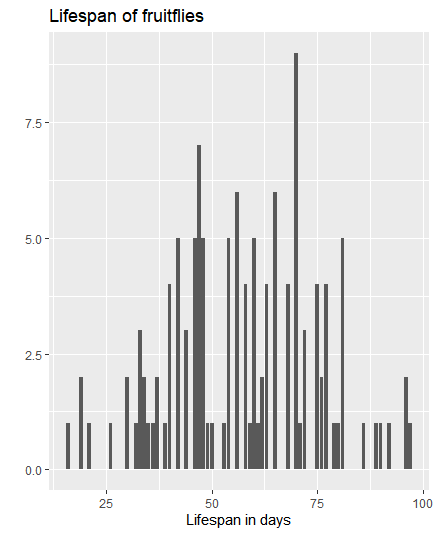
\includegraphics[width=\textwidth]{plot1}
	\caption{Lifespan of fruitflies}
	\label{fig:fruitflies}
\end{figure}

\subsection*{Task 2}
\textit{Plot \texttt{lifespan} vs \texttt{thorax}. Does it look like there is a linear relationship? Provide the plot. What is the correlation coefficient between these two variables?}

I am producing a scatterplot between the two variables, overlaid with a regression line and a confidence interval using ggplot. I also add the code line for the correlation coefficient here:

\lstinputlisting[language=R, firstline=69, lastline=74]{PS2_DW_R.R}

The correlation coefficient returned is \textbf{0.636}, hinting at a strong positive correlation between the two. The plot shown in Figure \ref{fig:thoraxlength} supports this idea; the regression line points clearly upwards with a relatively narrow confidence interval and the observated lifespans clearly increase.

\begin{figure}[h]
	\centering
	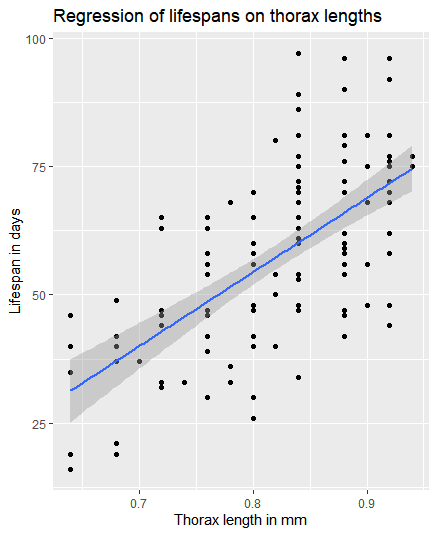
\includegraphics[width=\textwidth]{plot2}
	\caption{Lifespan of fruitflies and thorax length}
	\label{fig:thoraxlength}
\end{figure}

\subsection*{Task 3}
\textit{Regress \texttt{lifespan} on \texttt{thorax}.  Interpret the slope of the fitted model.}

\lstinputlisting[language=R, firstline=78, lastline=79]{PS2_DW_R.R}

The slope of the fitted model is returned as \textbf{144.33}. It should be remembered that this is the increase of the lifespan in days for an additional mm of thorax length; an increase that never occurs in real life as \ref*{fig:thoraxlength} shows: the range of thorax length lies between 0.64 and 0.94 mm. Still, this indicates a strong effect of thorax length on lifespan.

\subsection*{Task 4}
\textit{Test for a significant linear relationship between  \texttt{lifespan} and \texttt{thorax}. Provide and interpret your results of your test.}

In order to test a linear relationship, we first have to get a test statistic. The test statistic for a correlation is defined as $t = \frac{r\sqrt{n-2}}{\sqrt{1-r^2}}$; with n being 125 in this case. This gives us the following R code, returning a test statistic and a p-value through the pt() function:

\lstinputlisting[language=R, firstline=85, lastline=88]{PS2_DW_R.R}

This yields a p-value of $p = 7.484*10^-16$, an extremely low number suggesting that the association is not only strong, but also extremely significant.

\subsection*{Task 5}
\textit{Provide the 90\% confidence interval for the slope of the fitted model.}

\lstinputlisting[language=R, firstline=91, lastline=93]{PS2_DW_R.R}

In order to obtain the confidence interval, we have to calculate a margin of error using the qt() function. Dividing the desired p-value of 0.1 in half as we want a two-sided interval, we get a margin of error of 1.657 standard deviations. Multiplying this with the standard error derived from the regression object and adding and substracting it from the estimated slope - 144.33 - yields a confidence interval of \textbf{[118.197, 170.469]}. Using the confint() function yields the same result:

\lstinputlisting[language=R, firstline=95, lastline=95]{PS2_DW_R.R}

\subsection*{Task 6}
\textit{Use the \texttt{predict()} function in \texttt{R} to (1) predict an individual fruitfly's lifespan when \texttt{thorax}=0.8 and (2) the average \texttt{lifespan} of fruitflies when \texttt{thorax}=0.8 by the fitted model. This requires that you compute prediction and confidence intervals. What are the expected values of lifespan? What are the prediction and confidence intervals around the expected values?}

\lstinputlisting[language=R, firstline=99, lastline=101]{PS2_DW_R.R}

The expected values of lifespan in both cases are \textbf{54.415}. However, the confidence intervals are significantly wider in the prediction for an individual fruitfly, as they incorporate both the error in estimating the slope of the regression model and the error in picking an individual fruit fly. Therefore, the confidence interval for the average is \textbf{[51.91932, 56.91024]}, whereas it is  \textbf{[27.37542, 81.45414]} for an individual fruit fly.

\subsection*{Task 7}
For a sequence of \texttt{thorax} values, draw a plot with their fitted values for \texttt{lifespan}, as well as the prediction intervals and confidence intervals.

\lstinputlisting[language=R, firstline=105, lastline=115]{PS2_DW_R.R}

The code above produces a prediction for the values of 0.64 to 0.94, which equals the range of thorax lengths in the dataset. It does so in steps of 0.025 mm, resulting in 13 distinct predictions. Figure \ref{fig:predictions} then shows the line of predictions in a solid black line, the confidence interval for averages in dashed blue lines, and the confidence interval for a single prediction in dotted blue lines.

\begin{figure}[h]
	\centering
	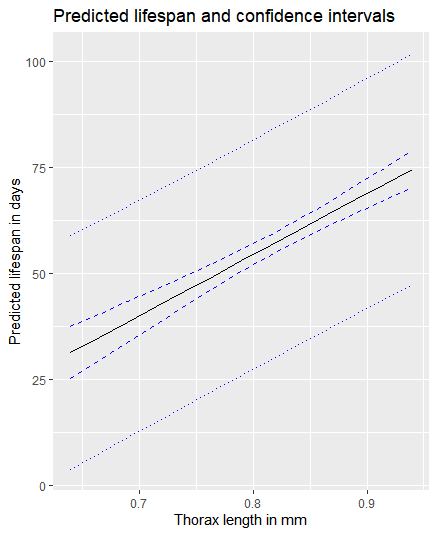
\includegraphics[width=\textwidth]{plot3}
	\caption{Predicted lifespan of fruitflies and thorax length}
	\label{fig:predictions}
\end{figure}

\end{document}